\chapter{A trait-based characterization of phytoplankton communities in contrasting environmental regions of the Atlantic Ocean}

\small {\textbf{Manuscript to be submitted to Marine Ecology Progress Series}}

%\subsection*{}
%\textbf{ABSTRACT}: In recent years trait-based ecology studies had been providing new insights on the mechanisms driving natural variation based on measurable key characteristics of organisms. Here we investigate the phytoplankton community size-composition in the Atlantic Ocean using data from the Atlantic Meridional Transect program. We extended the existing knowledge on the distribution of the phytoplankton size composition in the Atlantic, using a larger data set, integrating phytoplankton size composition, nutrients concentrations, and grazers abundance into a trait-based approach. The selected subset was constrain by k-means partitioning and based on the prevailing environmental conditions. Also we studied how the different phytoplankton size fractions respond to different environmental gradients. Our results suggest a linkage of the \textit{in situ} environmental conditions with community size-composition, and regardless of the spatio-temporal conditions. We discuss how the observed patterns of phytoplankton size-fractions in the Atlantic Ocean are coherent with the niche partitioning theory and opposed to the unified neutral theory of biodiversity.

\normalsize
\section{Introduction}
For decades ecologists have been trying to understand how the phytoplankton patterns of community structure are associated to the environmental conditions, with a particular focus on the causes and consequences of natural variations. One of the approaches adopted in this quest is based on observations of key characteristics of organisms, populations or communities. These key characteristics are also called traits \citep{McGill2006, Violle2007}. 

Trait-based ecology aims at developing an understanding and a better predictability of natural communities by linking traits that influence organism performances and fitness with prevailing environmental conditions \citep{McGill2006}. For example, recent investigations suggest that changes in mean trait and trait variance are invariable to different spatial scales, thus stressing the importance of the environmental conditions on trait variation and implying that the within-species and the interspecific variations on natural communities do not add more variation to the trait \citep{Messier2010}. 

Phytoplankton organisms are ideal systems for trait-based approaches. They are relatively simple with well defined ecological niches which are determined by the physical environment, the resource allocation strategies, and the interspecific relationships \citep{Litchman2007}. They have various morphological, physiological, behavioral and life history traits and trade-offs. Among all the known phytoplankton traits, cell-size is probably the best characterizing property of phytoplankton communities because many ecophysiological processes such as nutrient and light utilization and resistance to grazing, are significantly correlated with cell size \citep{Litchman2008,Litchman2010}. \textit{In vivo} and \textit{in situ} observations of a variety of traits are constantly measured due to the global importance of phytoplankton as primary producer, influencing trophic webs and biogeochemical cycles \citep{Falkowski1998}.

Almost every year, since 1995, two scientific cruises have been  crossing the Atlantic ocean from Plymouth (UK) to South America or South Africa, with observations including size fractionated chlorophyll-a, nitrate, phosphate and silicate concentrations, temperature and zooplankton abundances. These cruises are part of the Atlantic Meridional Transect Programme. Given the spatial extent of the transect, which crosses a range of ecosystems from sub-polar to tropical and from euphotic shelf seas and upwelling systems to oligotrophic mid-ocean gyres, the dataset is ideal for studying phytoplankton community structure and the driving processes of size composition at an ocean basin scale. Previous analyses attempted a description of the occurrences of the different size fractions \citep{Maranon2001} without considering a direct influence of the prevailing environmental conditions. A more comprehensive analysis that integrates all the different AMT data with the available phytoplankton community size-fractions is, to our knowledge, still lacking. Therefore, our work intends to uncover the mechanisms shaping the different phytoplankton community structures in regions of contrasting environmental conditions (that is: regions with different nutrient regimes and grazing pressures).

We broaden previous analyses by considering a larger selection of data than any previous study. More specifically, we integrate phytoplankton size-fractions with temperature, various nutrient concentrations, and zooplankton abundances in the attempt of disentangling the relative contribution of bottom-up and top-down processes in shaping phytoplankton size structure.

A first step in our analyses was to pre-structure the selected AMT dataset according to a well established ecological classification of marine data into ocean provinces characterised by different environmental conditions \citep{Longhurst2006}. In the second step, we propose a new classification using the available data of nutrient regimes and grazing, and compare our results with those of \citet{Longhurst2006}. In the last step, we relate the environmental differences and the relative contributions of bottom-up versus top-down processes to the different community size structures in order to highlight the emergent patterns of community compositions and structures at the ocean basin scale.

\section{Methods}

We composed a dataset by selecting a number of observed variables from the Atlantic Meridional Transect (AMT) Program (www.amt-uk.org). The resulting dataset comprises mixed-layer depth values of size fractionated chlorophyll-a, nitrate, phosphate and silicate concentrations, temperature, and zooplankton abundances (as a relative indication of grazing pressure). As mixed layer depth we considered that depth at which a variation of 0.5 $^\circ$C in temperature and of 0.125 in density is observed with respect to surface value (i.e. first value at 5-10 m depth). We obtained a dataset of 410 samples from a total of 9 AMT cruises (from AMT2 to AMT6, AMT10, AMT11, AMT13, AMT14). These cruises took place in April-May or September-October in the years 1996 (AMT2 and AMT3), 1997 (AMT4 and AMT5), 1998 (AMT6), 2000 (AMT10 -AMT11), and 2003 (AMT13 and AMT14). 

The phytoplankton size fractions available were in the range of picoplankton (0.2-2 $\mu$m), nanoplankton (2 -20 $\mu$m), and microplankon ($>$20 $\mu$m). AMT13 and AMT14 measured four size classes (0.2-2, 2-5 5-10, $>$10 $\mu$m). Thus, to be consistent with the three plankton size ranges, we considered the 2-5 and 5-10 $\mu$m size classes as part of the nanoplankton class and the $>$10 $\mu$m class as part of the microplankton class. We checked for the results with and without these data and there was no appreciable difference in the resulting patterns. The three size fractions were normalized, based on the proportion of each size fraction to the total Chl-a concentration.

\begin{wrapfigure}{r}{0.5\textwidth}
\begin{center}
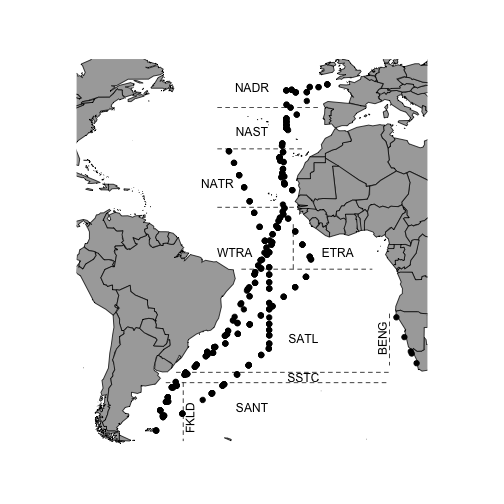
\includegraphics[trim = 30mm 20mm 25mm 20mm, clip, width=1\linewidth]{./Chp2-Pre/amt_mapFINAL2.png}
\end{center}
\caption[Scheme]{\small {The AMT subset of 410 samples used on this study. The dashed lines represent the simplified limits of the Longhurst (2006) ecological provinces.}}
\label{Map}
\end{wrapfigure}

The selected dataset covers temperate, subtropical and tropical regions of the Atlantic ocean (Figure \ref{Map}). According to Longhurst's (\citeyear{Longhurst2006}) classification, ten ecological provinces were sampled by these cruises: four temperate provinces, comprising the North Atlantic Drift (NADR; n=24), the South Subtropical Convergence (SSTC, n=21), the Subantartic Water Ring (SANT, n=14), and the Falkland Island (FKLD; n=52); two subtropical provinces, comprising the North Atlantic Subtropical Gyral (NAST; n=37) and the South Atlantic Subtropical Gyral (SATL, n=129); three tropical provinces, the North Atlantic Tropical Gyral (NATR, n=51), the Eastern Tropical Atlantic (ETRA, n=13) and the Western Tropical Atlantic (WTRA, n=64); and one upwelling region, the Benguela province (BENG, n=5). With this dataset we analyzed the phytoplankton community size composition and implemented a linear mixed effect model (LME) to test if the community size-structure differs among ecological provinces. The ecological provinces were classified by regions, defined as: temperate (NADR, FKLD, SSTC, SANT), tropical (NATR, WTRA, ETRA), subtropical (SATL, NAST) and upwelling (BENG). The model was fitted to the data using the size fractions and the regions as fixed factors, and the ecological provinces as random factors.

We utilized a cluster analysis based on k-means partitioning to alternatively classify the data according to the prevailing environmental conditions. The environmental variables considered were nitrate + nitrite concentration, phosphate concentration, silicate concentration and temperature. We performed a principal component analysis (PCA) of the environmental variables and the normalized size fractions to assess the relative importance of a specific environmental gradient to the phytoplankton size fractions. We quantified the linear relationships between the environmental and the community size-structure. In addition we also quantified the response of the three size fractions to the grazer abundance, but only using data of the cruises AMT3 and AMT5, due to a limited availability of the zooplankton data. These analyses were carried out using R v2.12.2 (The R Foundation for Statistical Computing, 2011).

\section{Results}

\begin{figure}
\centering
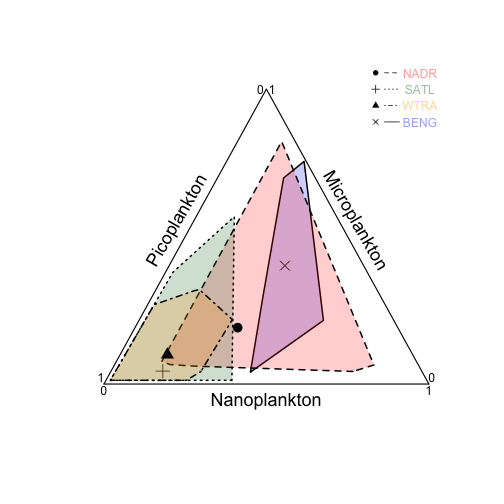
\includegraphics[trim = 20mm 30mm 20mm 20mm, clip, width=0.5\linewidth]{./Chp2-Pre/amt_4RegionsTriSizeFrac4.png}
\caption[Scheme]{\small {Phytoplankton community size structure of four ecological provinces in the Atlantic Ocean.The contours correspond to the convex hull of the size-fractions distribution on each province and the symbols denotes the mean values.}}
\label{RegSizeFrac}
\end{figure}

\begin{figure}
\centering
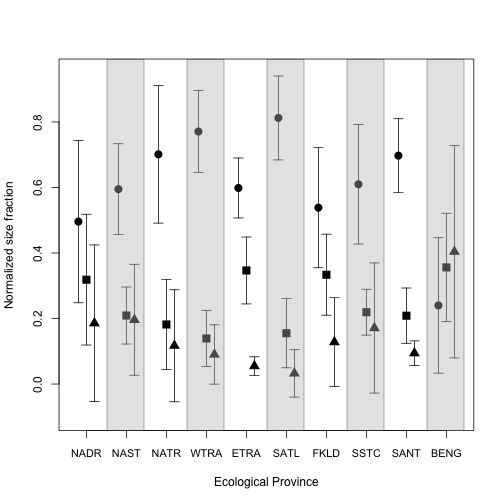
\includegraphics[trim = 0mm 0mm 0mm 0mm, clip, width=0.8\linewidth]{./Chp2-Pre/amt_MeanSDProvinces.png}
\caption[Scheme]{\small {Mean values ($\pm$sd) of three phytoplankton size fractions in ten ecological provinces of the Atlantic Ocean. The symbols indicate the means of the normalized size fractions of: picoplankton (\ding{108}), nanoplankton(\ding{110}) and microplankton (\ding{115}).}}
\label{means}
\end{figure}

Community size-structure is highly variable in different ecological provinces. (Figure \ref{RegSizeFrac}). When the mean size-fraction values of only four selected provinces are compared, an increasing trend towards bigger phytoplankton sizes can be observed from the warmer provinces in the tropics and subtropics to the colder provinces in the Benguela upwelling. In tropical and subtropical waters (such as WTRA and SATL), picoplankton is the most common size class, with only a few occurrences of nano- and microplankton. Temperate provinces such as NADR are characterised by a more heterogeneous distribution of size classes. By contrast, the upwelling province  shows a distribution of size fractions dominated mainly by pico- and microplankton. Provinces located in the temperate regions appear to show a larger cell size variability, as indicated by a broader standard deviation, when compared to provinces located in the tropical regions (Figure \ref{means}). These differences are significant for the picoplankton (LME/anova, df=3, F=6.6315, p=0.0247) and the microplankton size fractions (LME/anova, df=3, F=5.5189,p=0.0368), while they are less significant for the nanoplankton (LME/anova, df=3, F=2.03341, p=0.2108).

\begin{figure}
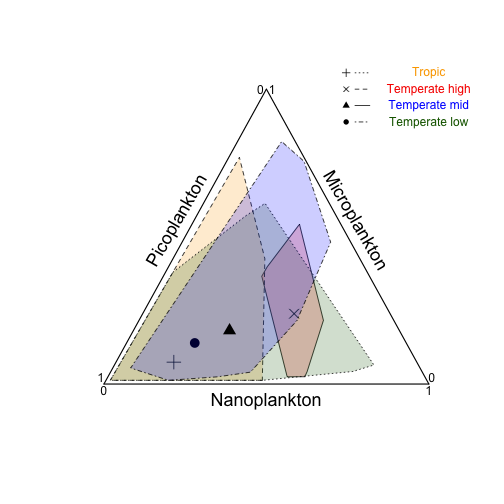
\includegraphics[trim = 12mm 15mm 10mm 15mm, clip, width=0.5\linewidth]{./Chp2-Pre/amt_clsEnvFINAL4.png}
\put(1,210){\textbf{b)}}
\put(-180,210){\textbf{a)}}
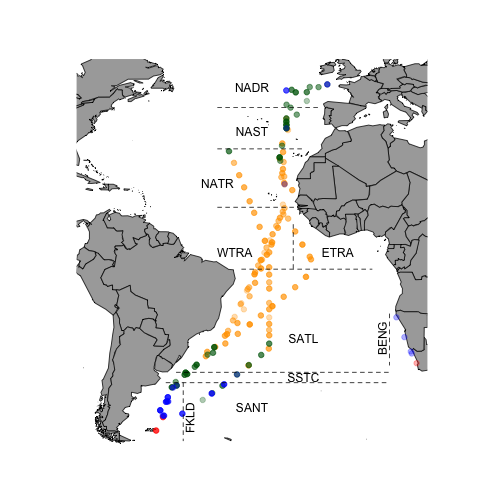
\includegraphics[trim = 20mm 20mm 20mm 20mm, clip, width=0.5\linewidth]{./Chp2-Pre/amt_mapClsEnv3.png}
\caption[Scheme]{\small {Phytoplankton community size structure as function of environmental conditions. a)Distributions of size-classes clustered according to Tropic and Temperate conditions with low, mid and high nutrient concentration, with contours corresponding to the convex hull of the size-fractions distribution on each cluster and symbols denoting the mean values. b)Geographical distribution of the clusters compared with Longhurst classification, with color-coding reflecting the cluster classification.}}
\label{clusters}
\end{figure}

\begin{table}
\centering
\caption[Scheme]{\small {Mean values of environmental data for the different clusters with low mid and high referring to the amount of nutrient concentration.}}
\label{tableclus}
\begin{tabular} {c c c c c}
cluster & $NO_2^-$ + $NO_3^-$ & $PO_4^{3-}$ & $SiO_4^{2-}$ & Temperature \\ \hline
Tropic & 0.150$\pm$0.575 & 0.064$\pm$0.078 & 1.097$\pm$0.575 & 25.299$\pm$2.000 \\
Temperate low & 0.556$\pm$1.102 & 0.112$\pm$0.141 & 0.816$\pm$0.617 & 17.894$\pm$2.191 \\
Temperate mid & 9.027$\pm$3.593 & 0.799$\pm$0.373 & 2.423$\pm$1.375 & 11.925$\pm$2.797 \\
Temperate high & 30.324$\pm$4.549 & 1.336$\pm$0.208 & 4.590$\pm$1.926 & 6.810$\pm$3.435 \\ \hline
\end{tabular}
\end{table}

Our k-means clustering analysis of temperature, nitrate, phosphate, and silicate concentrations on all provinces show that tropical and subtropical regions share the same environmental characteristics (yellow dots in Figure 2.4b and see also Table 2.1), while temperate provinces are different and are categorized into three main regions: temperate low, temperate mid and temperate high (respectively green, blue and red dots in Figure 2.4b, and see also Table 2.1). In summary, we obtained a new classification of the data into four regions, which explains 87.3\,\% of variance. The mean phytoplankton size compositions of the new four clusters show (Figure 2.4a) an increasing trend from the high-temperature, low-nutrient regions (tropic) towards the low-temperature, high-nutrient regions (temperate). A principal component analysis of all data shows highest loadings for temperature (positive loading) and nitrate concentration (negative loading) with respect to the first principal component (Figure \ref{PrinComp}). Furthermore, the picoplankton size fraction positively correlated with temperature while nutrient concentrations are positively correlated with nano- and microplankton size fractions (Figure \ref{PrinComp}).

A regression analysis of all the data shows that phytoplankton size composition varies with the environmental conditions irrespective of temporal changes (see Figure \ref{response1} and Table \ref{stats}). A shift from a picoplankton dominated community towards a nano- and microplankton dominated community occurs at increasing in nutrient concentrations (see Figure \ref{response1}a, \ref{response1}b and \ref{response1}c). By contrast, at increasing temperature the relative proportion of picoplankton increases from about 40\% to about 80\%, while the nano- and microplankton are both reduce by about 50\%.

When restricting our regression analysis to data of the only two cruises (AMT3 and AMT5) that sampled zooplankton,we can observe that an increase in copepods abundance corresponds to a decline in picoplankton from 70$\%$ to less than 40$\%$, to an increase in nanoplankton from 20$\%$ to 60$\%$, and to no appreciable change in microplankton (Figure \ref{response2}).

\begin{figure}
\centering
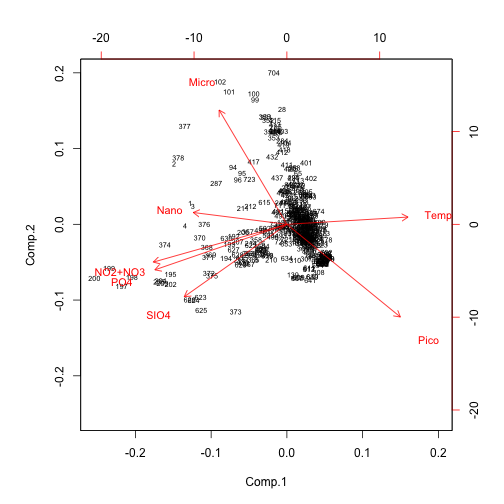
\includegraphics[trim = 0mm 0mm 0mm 0mm, clip, width=0.9\linewidth]{./Chp2-Pre/amt_PrinComp.png}
\caption[Scheme]{\small {Principal component analysis of environmental conditions and normalized phytoplankton size fractions.}}
\label{PrinComp}
\end{figure}

\begin{figure}
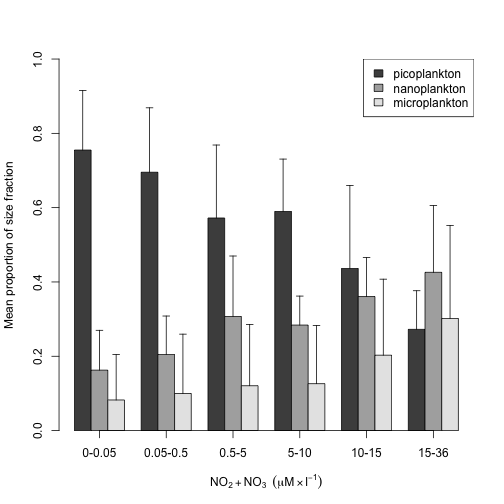
\includegraphics[trim = 0mm 0mm 0mm 15mm, clip, width=0.5\linewidth]{./Chp2-Pre/amt_NO3_bars2.png}
\put(-180,210){\textbf{a)}}
\put(1,210){\textbf{b)}}
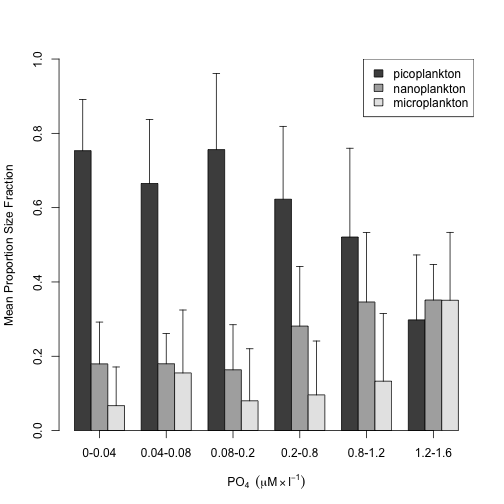
\includegraphics[trim = 0mm 0mm 0mm 15mm, clip, width=0.5\linewidth]{./Chp2-Pre/amt_PO4_bars2.png}
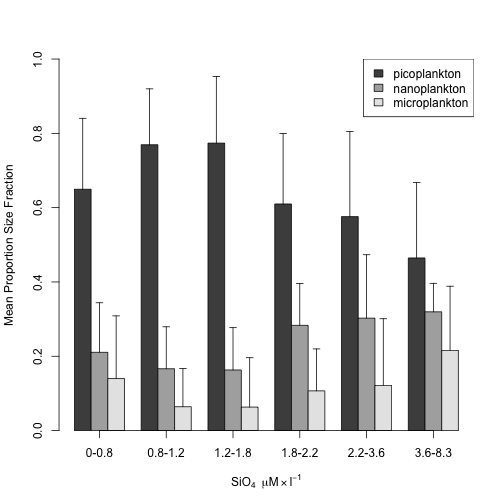
\includegraphics[trim = 0mm 0mm 0mm 15mm, clip, width=0.5\linewidth]{./Chp2-Pre/amt_SiO4_bars2.png}
\put(-180,210){\textbf{c)}}
\put(1,210){\textbf{d)}}
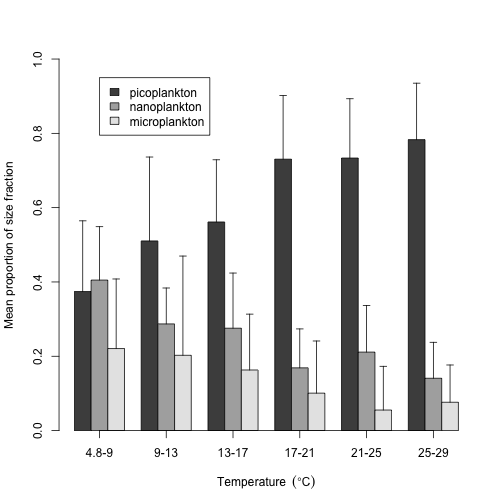
\includegraphics[trim = 0mm 0mm 0mm 15mm, clip, width=0.5\linewidth]{./Chp2-Pre/amt_Temp_bars2.png}
\caption[Scheme]{\small {Response of picoplankton, nanoplankton and microplankton size fraction to nitrite+nitrate, phosphate, silicate and temperature. Bars represent mean values and the error bars the standard deviation.}}
\label{response1}
\end{figure}

\begin{figure}
\centering
\includegraphics[trim = 0mm 0mm 0mm 15mm, clip, width=0.6\linewidth]{./Chp2-Pre/amt_zoo_bars2.png}
\caption[Scheme]{\small {Response of picoplankton, nanoplankton and microplankton size fraction to copepod abundance. Bars represent mean values and the error bars the standard deviation.}}
\label{response2}
\end{figure}

\begin{table}
\centering
\caption[Scheme]{\small {Summary statistics of linear fitting for the response of three size fractions to each environmental variable}}
\label{stats}
\begin{tabular} {c c c c c c c c c c }
& \multicolumn{3} {c} {Picoplankton} & \multicolumn{3} {c} {Nanoplankton} & \multicolumn{3} {c} {Microplankton} \\
& slope & p-value & $r^2$ & slope & p-value & $r^2$ & slope & p-value & $r^2$ \\ \hline
$NO_2^-$+$NO_3^-$ &-0.090 &0.002 & 0.908 &0.050 &0.001 & 0.921 &0.040 &0.010 &0.792 \\
$PO_4^{3-}$ &-0.0812 &0.021 &0.711 &0.042 &0.012 &0.777 &0.039 &0.125 &0.354 \\
$SiO_4^{2-}$ &-0.047 &0.085 &0.455 &0.030 &0.044 &0.597 &0.016 &0.247 &0.142 \\ 
Temperature &0.082 &0.001 &0.914 &-0.047 &0.008 &0.812 &-0.035 &0.003 &0.885 \\
Copepods &-0.063 &0.064 &0.520 &0.068 &0.051 &0.567 &-0.004 &0.788 &-0.222\\ \hline
\end{tabular}
\end{table}


\section{Discussion}
We analysed different data from different AMT cruises, covering mainly two seasons (late spring/early summer and autumn) from 1996 to 2003 and from different areas of the Atlantic Ocean. Our results showed patterns of phytoplankton size distributions characterized by the dominance of picoplankton in oligotrophic (SATL) and tropical (e.g. WTRA) waters and by the dominance of larger size classes in nutrient-rich waters (BENG), consistently with \citet{Maranon2000, Maranon2001, Poulton2006, Moreno-Ostos2011, Huete-Ortega2011}. These phytoplankton size compositions resulted to be strongly associated with changes in environmental conditions (Figures 2.6 and 2.7). The consistency of our results with similar previous studies of the Atlantic Ocean but that used either less AMT data than our study \citep{Maranon2000, Maranon2001, Poulton2006} or data from sources different than the AMT cruises \citep{Moreno-Ostos2011, Huete-Ortega2011} suggests that the different phytoplankton size structures observed are robust features of the Atlantic Ocean. 

The differences in size-fractions we found in regions of contrasting environmental characteristics (tropical versus temperate) support the view \citep{Messier2010} that environmental conditions strongly influence the trait distribution (cell size in our case). 

Comparing the results of our classification approach with the one of Longhurst, we note that the classification in ecological regions made by Longhurst make a better contrast of the size-structures in the different ecological provinces. This may be due to the higher temporal and spatial resolution of the environmental data used by Longhurst. However, the increased trend of the mean values is a feature that is well capture by both approaches.

The results we obtained with the clustering technique (Figure \ref{clusters}) suggest that the areas between 30$^\circ$ N and 30$^\circ$ S are characterize by nutrient and temperature regimes favouring communities with higher proportions of picoplankton size classes. The temperate areas laying at the edges of this region are distinguished by colder waters and higher nutrient concentrations and by a wider range of phytoplankton size class. It is well known that stronger seasonal changes in the temperate areas lead to these shifts in the community composition. 

From our regression analyses (Figures \ref{response1} and \ref{response2}) we inferred a strong control of NO$_3^-$+NO$_2^-$ and temperature on all three size fractions. While only pico- and nanoplankton size fractions appear to significantly respond to changes in PO$_4^{3-}$, SiO$_4^{2-}$ and copepod abundance. These strong controls could be explained by the trade-offs between resource acquisition and predation pressure leading to specific size classes dominating the phytoplankton community under given environmental conditions. For example, smaller phytoplankton cell sizes have a competitive advantage over larger phytoplankton under low nutrient, low light and low grazing pressure \citep{Litchman2008, Litchman2010}. There are also a number of important physiological and ecological processes that strongly depend on phytoplankton cell size \citep{Kiorboe1993, Cermeno2008a, Finkel2009a}, including metabolic rates, maximum nutrient uptake rate, nutrient diffusion, light absorption, sinking velocity, trophic interactions and even diversity within taxa, which  is often a log-normal distribution of body size. Our results are therefore consistent with this general "size rules" \citep{Finkel2009a}, although to our knowledge this is the first time that such aspects are observed in data extending across an entire ocean basin and irrespective of the temporal changes.

In summary our size-based analyses substantiates some remarkable feature concerning the variation of a key trait such as cell size at an ocean basin scale, and irrespective of temporal changes. Moreover, these findings are consistent with Baas Becking's tenet "everything is everywhere, but the environment selects" \citep{BaasBecking1934, DeWit2006,O'Malley2007}, over large-scale environmental changes. However, the hypothesis that the prevailing environmental conditions are the major driving forces of the phytoplankton community structure in the Atlantic Ocean should be further investigated using the trait-based modelling approach of  \citet{Bruggeman2007, Merico2009}, a research direction also promoted very recently by \citet{Follows2011}. This modelling approach will further stimulate the development of a theoretical framework for exploring in detail the effects of large-scale environmental differences on planktonic communities.

\section{Acknowledgements}
This study uses data from the Atlantic Meridional Transect Consortium (NER/0\\/5/2001/00680), provided by the British Oceanographic Data Centre and supported by the Natural Environment Research Council. 
